\documentclass[11pt,a4paper]{article}

\usepackage[margin=1.5in]{geometry}
\usepackage[utf8]{inputenc}
\usepackage[english]{babel}
\usepackage[T1]{fontenc}
\usepackage{lmodern}
\usepackage{mathtools}
\usepackage{subcaption}
\usepackage{float}

\usepackage{amsmath,amssymb,amsfonts}

\DeclarePairedDelimiter{\ceil}{\lceil}{\rceil}
\DeclarePairedDelimiter{\floor}{\lfloor}{\rfloor}

\title{Vision and Image Processing\\Assignment 1}
\author{Malte Stær Nissen}

\begin{document}
\maketitle

\section{Detecting interest points}
The detection of interest points can be made by utilizing a variety of methods. I
have implemented\footnote{The entire implementation of this assignment is made
in Matlab R2013b.} both the two blob detectors Difference of Gaussians (DoG) and
Laplacian of Gaussian (LoG) as well as the Harris corner detector. All three detectors
are implemented by hand only using simple Matlab standard functions.
Throughout this report I1 references the image
\texttt{Img\_001\_diffuse\_smallgray.png}, I2 references
\texttt{Img\_002\_diffuse\_smallgray.png} and I3 references
\texttt{Img\_009\_diffuse\_smallgray.png}.

\subsection{Blob detectors}
Both blob detectors are implemented by first creating either a DoG or LoG
filter. These filters are created by sampling the appropriate Gaussian
distribution(s) (and their derrivatives) with a support radius of $3\sigma$
and hence a filter size of $\ceil{6 \sigma} \times \ceil{6\sigma}$ in order to
get a sufficient part of the distribution included in the filter. The second
part of the blob detectors is to perform a simple convolution of an image with
the filter just found. The boundary cases are handled by using replication of
boundary pixels to avoid the padding to contribute to the derrivatives. The
third and last part of the blob detectors is to find local extrema (maxima and
minima only) in the convolved image using either 4- or 8-connectivity (I use
8 in all included examples) and leave out extremas below (using the absolute
value of the extremas) a certain threshold $t$.

\subsection{Harris corner detector}
The Harris corner detector is likewise implemented by computing derrivatives
of the Gaussian distribution, filtering appropriately and then computing the
Harris corner measure followed by a local maxima search and thresholding using
threshold $t$.

I considered whether to extend one of my implemented filters to a multi-scale
version er not, which would probably give better results. Given the timeframe
for the assignment and my choice of implementing all three detectors I chose
not to extend any of them to multi-scale. This could however be done by a
relatively simple loop over a finite set of scales registering the scale for each
interesting point and taking care of the change to either 6- or 26-connectivity
(across neighbour scales as well).

\subsection{Results and parameters}
Figure \ref{fig:i1_points} and \ref{fig:i4_points} shows the 50 most
significant interest points of running each of the three point detectors on
the images I1 and \texttt{tiles.jpg}. The red crosses, green circles and
yellow squares mark the LoG, DoG and Harris results respectively. The LoG and
DoG points are selected by choosing the 25 most significant light and 25 most
significant dark points. The selection of points is however only made in order
to visually determine the outcome of the algorithms.

For figure \ref{fig:i1_points} I've used $\sigma = 5.28$ and an absolute
threshold of $0.008$ (original image converted to double precision in the
range 0 to 1) for the LoG detector. For the DoG detector I've used $\sigma =
2,~k = 8$ and an absolute threshold of 0.15. For the Harris corner detection
I've used $\sigma = 0.88,~k=5,~\alpha = 0.1$ and $t= 0.5\cdot
10^{-5}$.

For figure \ref{fig:i4_points} I've used $\sigma = 10$ and $t= 0.0005$ for
LoG, $\sigma = 2,~k=5$ and $t = 0.001$ for DoG, and $\sigma = 2,~k=10$ and $t=
0.5\cdot 10^{-8}$ for the Harris detector.

We first comment on figure \ref{fig:i1_points}. As expected the Harris corner
detection finds points that are clearly having corners in their neighbourhoods
whereas the blob detectors tend to find both corner points as well as blobs
and lines. This can especially be seen at the second rooftop from the left
where the LoG detector finds a series of blobs on the rooftop line as well as
the DoG detector finding a similar series of points in the two windows at the
bottom of one of the houses. Both of these are equally finding a lot of points
on the left-most car, where the Harris detector only finds three corners.

Figure \ref{fig:i4_points} displays the problem when using single-scale
detectors. The detectors are finding somewhat fine interesting points in the
middle of the image (vertical middle). At the bottom of the image both the LoG
and Harris detectors are identifying a lot of the coarser ``noise'' in the tiles
as interesting points. If we are only interested in finding corners/edges of the
tiles these points should ideally be removed. Likewise the algorithms fail to
identify the corners of the tiles at the top left part of the image. Having used
a multiscale detector, we could potentially both have left out many of the
points at the bottom and allowed the detector to keep interesting points in the
top. I am however not able to substantiate this thought as I haven't implemented
a multiscale detector.

\begin{figure}[h]
    \centering
    \begin{subfigure}[t]{0.8\textwidth}
        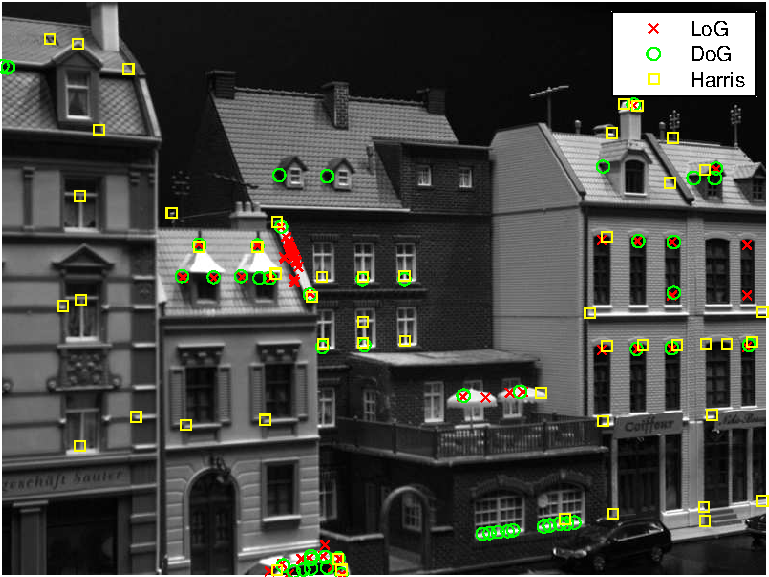
\includegraphics[width=\textwidth]{images/i1_points.pdf}
        \caption{I1 results}
        \label{fig:i1_points}
    \end{subfigure}
    \begin{subfigure}[t]{0.8\textwidth}
        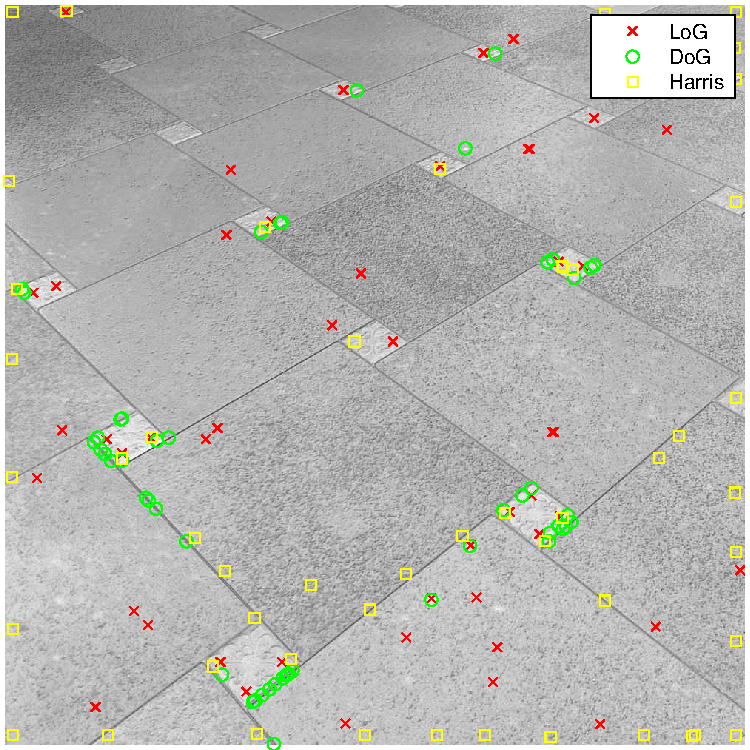
\includegraphics[width=\textwidth]{images/i4_points.pdf}
        \caption{\texttt{tiles.jpg} results}
        \label{fig:i4_points}
    \end{subfigure}
    \caption{Plot of the 50 most significant interest points using the LoG
    (red crosses), DoG (green circles), and Harris (yellow squares) detector.}
\end{figure}

\section{Simple matching of features}
The simple matching of features is implemented by using the normalized cross
correlation (NCC) dissimilarity measure on patches from the two images we want
to match points from. Having two images with interest points already detected
we match the points by running through the list of points from the one image
and match it with the interest point from the second image having NCC value
closest to 0. Furthermore we check if the ratio between the best and 2nd
best match is below a threshold $t$ and throw away the match if this check
fails. This is done in order to try to prevent insecure matches from being
registered. If the ratio is above the threshold, the two patches/matches
are expected to be quite similar ``distance'' from eachother. This could
be because of all patches matching poorly or two possible patches being so
similar that we cannot decide which one to use. For this assignment I use
$t = 0.8$ since this has shown to give somewhat good results by manually
experimenting with the parameter. It should be mentioned that I have chosen to
zero-pad patches when looking at interest points close enough to the borders for
the patches to extend outside the image. Furthermore when mapping multiple
points from one image to a single point in the second, we could choose to keep
only the best match. I have however ommitted this from my implementation.

I have chosen to use the Harris detection points (and the same setup as for
figure \ref{fig:i1_points}) for testing out the matching of features in this
report. Figure \ref{fig:matches} visualizes matching points between the pairs
I1, I2 (figures \ref{fig:i1_i2_harris_11} and\ref{fig:i1_i2_harris_51}) and
I1,I3 (figures \ref{fig:i1_i3_harris_11} and \ref{fig:i1_i3_harris_51}) using
patch sizes of $11\times11$ and $51\times51$.

Since the images are more or less purely having a horizontal rotation in the
view and we don't have a ground truth, the easiest way of quantifying the
performance of a match is by visual inspection. Horizontal lines are often
correct matches and non-horizontal lines are often incorrect. By inspecting
figures \ref{fig:i1_i2_harris_11} and \ref{fig:i1_i2_harris_51} we see that the
matching between I1 and I2 looks to be better (almost all points are matched
with their correct counterpart) when using a patch size of
$51\times51$ instead of $11\times11$. The use of a bigger patch size is however
affecting the performance when looking at matches between I1 and I3 in figures
\ref{fig:i1_i3_harris_11} and \ref{fig:i1_i3_harris_51}. There is a smaller
amount of non-horizontal lines when using $51\times51$ sized patches than for
$11\times11$ sized patches. There are however also some points that were
correctly matched using the smaller patches which disappears when using the
bigger patches.

The performance is bound to decrease since a larger variation in the view angle between
the two images naturally change the lighting and view of the physical objects.
This will in terms change the shapes captured by the camera. Furthermore some
previously captured interest points could be hidden due to the angle change
and new interest points could likewise be revealed. All these changes make it
harder for our matching algorithm as the optimal patch matches decrease in
similarity and hence we are prone to erroneous matching. This is however because
we are using the raw pixels to compare points to one another. Instead of using the
NCC dissimilarity measure on raw pixels we could potentially use an
implementation of the SIFT measure to compare patches while keeping the rest of
the comparison algorithm.

\begin{figure}[h]
    \centering
    \begin{subfigure}[t]{0.9\textwidth}
        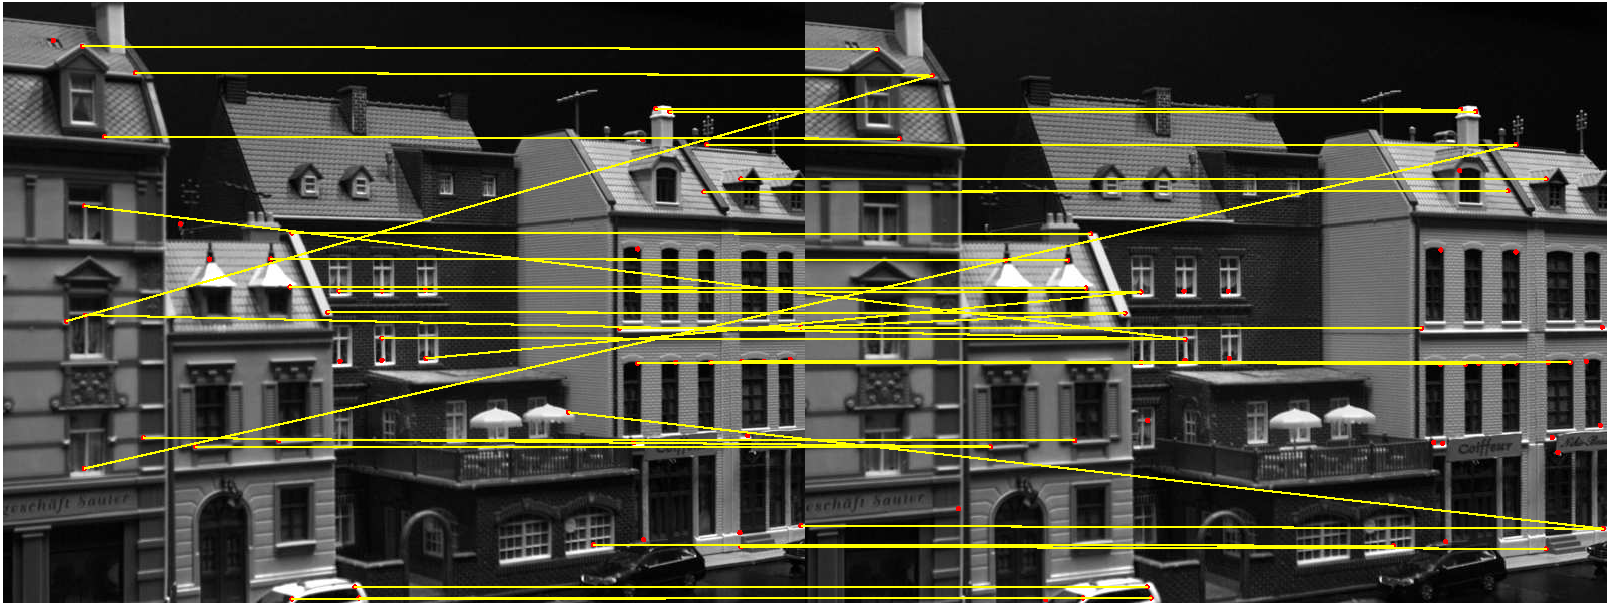
\includegraphics[width=\textwidth]{images/match_i1_i2_harris.pdf}
        \caption{I1 and I2, patch size $11\times11$}
        \label{fig:i1_i2_harris_11}
    \end{subfigure}
    \begin{subfigure}[t]{0.9\textwidth}
        \centering
        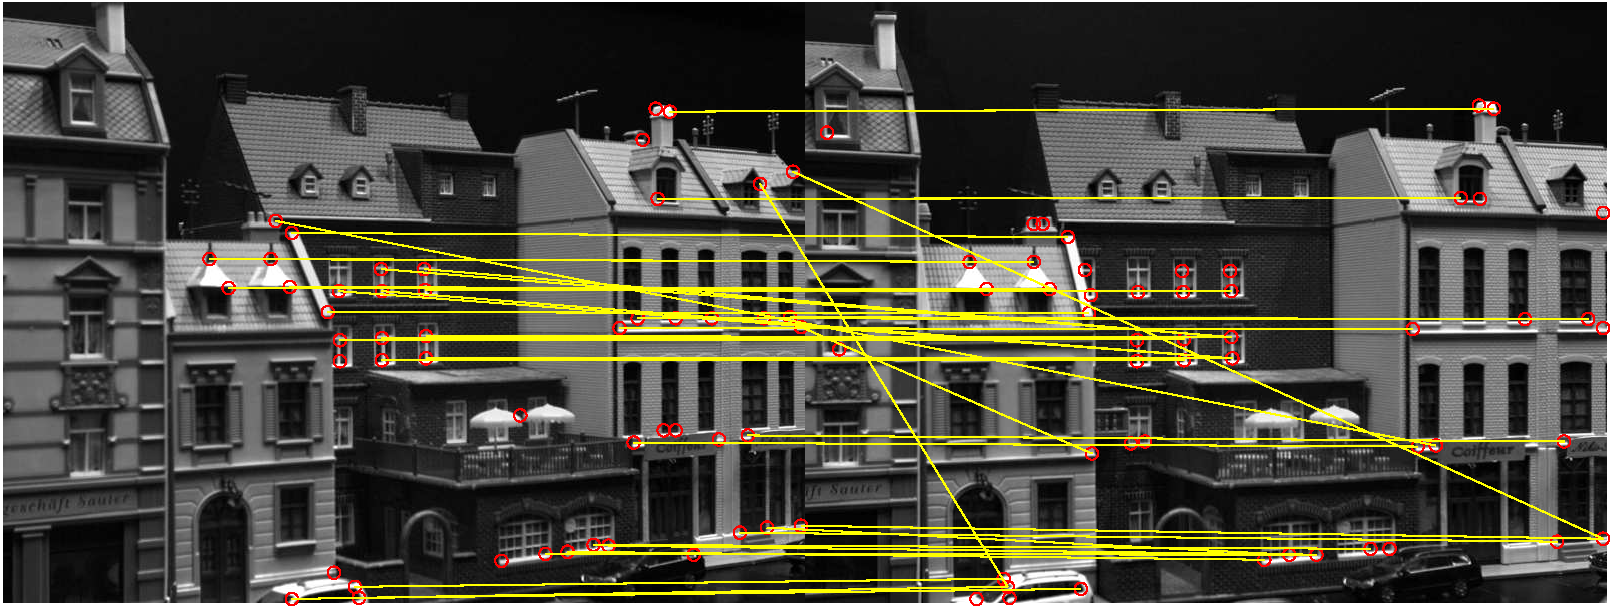
\includegraphics[width=\textwidth]{images/match_i1_i3_harris.pdf}
        \caption{I1 and I3, patch size $11\times11$}
        \label{fig:i1_i3_harris_11}
    \end{subfigure}
    \begin{subfigure}[t]{0.9\textwidth}
        \centering
        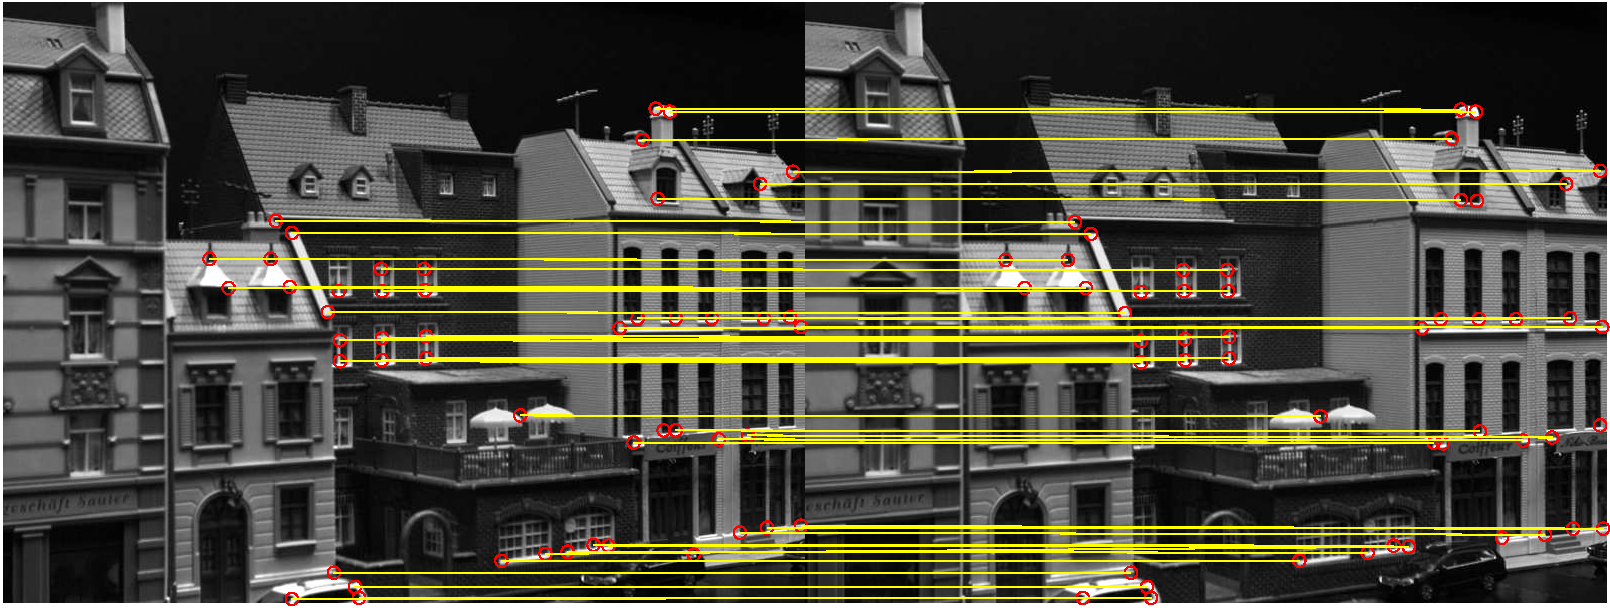
\includegraphics[width=\textwidth]{images/match_i1_i2_harris_51.pdf}
        \caption{I1 and I2, patch size $51\times51$}
        \label{fig:i1_i2_harris_51}
    \end{subfigure}
    \begin{subfigure}[t]{0.9\textwidth}
        \centering
        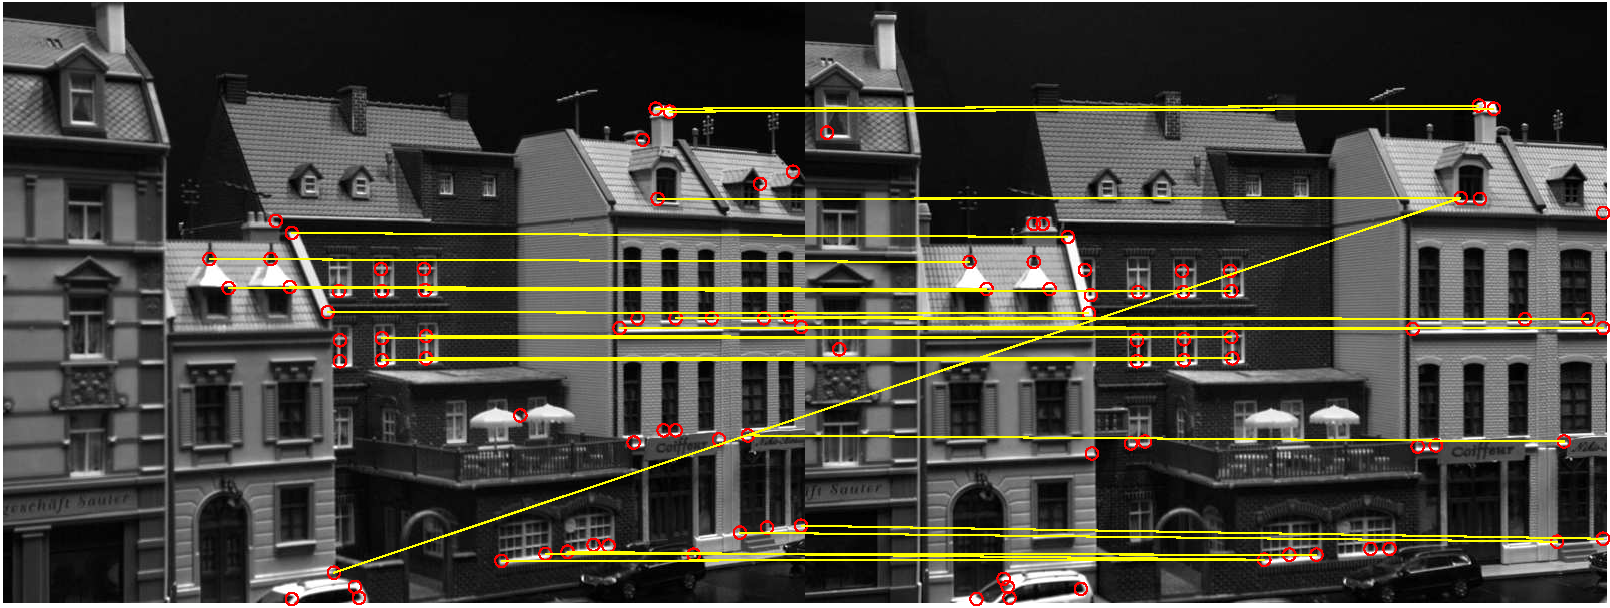
\includegraphics[width=\textwidth]{images/match_i1_i3_harris_51.pdf}
        \caption{I1 and I3, patch size $51\times51$}
        \label{fig:i1_i3_harris_51}
    \end{subfigure}
    \caption{Harris corners matches using NCC on raw pixel data.}
    \label{fig:matches}
\end{figure}

\end{document}
